% Created 2022-06-20 Mon 17:56
% Intended LaTeX compiler: pdflatex
\documentclass[11pt]{article}
\usepackage[utf8]{inputenc}
\usepackage[T1]{fontenc}
\usepackage{graphicx}
\usepackage{longtable}
\usepackage{wrapfig}
\usepackage{rotating}
\usepackage[normalem]{ulem}
\usepackage{amsmath}
\usepackage{amssymb}
\usepackage{capt-of}
\usepackage{hyperref}
\author{Youssef}
\date{\today}
\title{Les Médicaments à Status Particulier}
\hypersetup{
 pdfauthor={Youssef},
 pdftitle={Les Médicaments à Status Particulier},
 pdfkeywords={},
 pdfsubject={},
 pdfcreator={Emacs 28.1 (Org mode 9.5.4)}, 
 pdflang={English}}
\begin{document}

\maketitle
\tableofcontents

\setlength{\parindent}{0pt}

\section{Stupéfiants}
\label{sec:orgbbf85bd}
Une prescription de stupéfiant doit contenir la dose et la posologie.
Le patient à \textbf{72 heures} pour recevoir une dispensation complète de son traitement\footnote{Sinon il faudra déconditionner}.

Le pharmacien doit les stocker dans une armoire \textbf{fermée à clef différente} de celle des stupéfiants détenus à l'officine

Le transport à l'étranger pour un patient doit se faire par une \textbf{autorisation de transport de l'ARS locale au médecin prescripteur}.

La morphine injectable peut être prescripte pour \textbf{7 jours} maximum.

La délivrance de FENTANYL \emph{adm: patch, buccale, ou nasale} pour les douleurs chroniques doit être fractionnée \textbf{sauf mention expresse du prescripteur}

La Méthadone peut être prescrite jusqu'à \textbf{28 jours}, et délivrée par fractions de \textbf{7 jours} sauf mention expresse du prescripteur.

\subsection{Ordonnance}
\label{sec:org0e06452}
\begin{itemize}
\item Sécurisée
\item Doit afficher \emph{en toutes lettres}:
\begin{itemize}
\item le nombre d'unité par prise
\item Nombre de prise
\item dosage
\end{itemize}
\end{itemize}

\begin{center}
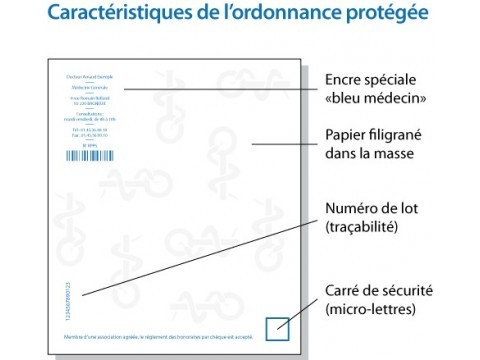
\includegraphics[width=.9\linewidth]{./ordo_securisee.png}
\end{center}

\subsection{Délivrance}
\label{sec:orge4a0bf0}
\begin{center}
\begin{tabular}{lll}
DCI & Fractionnement & Exemples\\
\hline
Fentanyl \emph{transdermique} & 14 j & Durogesic, Matrifen\\
Fentanyl \emph{transmuqueuse} & 7 j & Actiq, Effentora, Abstral, Instanyl, Pecfent\\
Methadone & 7 j & \\
\end{tabular}
\end{center}

\subsection{Mentions à Apposer}
\label{sec:orgdc2e6a3}
\begin{itemize}
\item Tampon de l'officine
\item N° enregistrement sur l'ordonnancier
\item Date de délivrance
\item Nom de la spécialité délivrée
\item Quantité délivrée en unité de prise
\end{itemize}

\subsection{Comptabilité et Traçabilité}
\label{sec:org0c5d62d}
\begin{itemize}
\item Comptabilité journalière
\item Balance mensuelle
\item Inventaire annuel du stock
\item Conservation des ordonnances pendant 10 ans
\end{itemize}

\section{Assimilés Stupéfiants}
\label{sec:org9654a42}
Ils sont prescrits sur une ordonnance sécurisée, et sont stockés dans un lieu avec accès restreint.
Le patient à 3 mois pour reçevoir la totalité de sa prescription\footnote{Pas de déconditionnement possible.}.

La durée de prescription maximale dépend du médicament, fixée par arrêté ministériel.

Tous les AS \footnote{Assimilé stupéfiant} ne sont pas renouvellables.

\section{Anxiolytiques et Hypnotiques}
\label{sec:orgc0c256f}

\subsection{Première délivrance}
\label{sec:orgf91653a}
Elle se fait uniquement sur une ordonnance datant de moins de 3 mois.

\subsection{Prescription et Règles de Délivrance}
\label{sec:org7149e8f}
\begin{center}
\begin{tabular}{ll}
Hypnotiques & 4 semaines\\
Anxiolytiques & 12 semaines\\
\end{tabular}
\end{center}

\emph{Il est interdit de renouveller de manière exceptionnelle un anxiolytique ou hypnotique}

\section{Médicaments d'Exception}
\label{sec:org6b1ab79}
Ce sont des spécialités remboursées uniquement pour certaines indications.
Leur prescription se fait alors sur une ordonnance 4 volets\footnote{Conforme au Cerfa 12708*02}.

\begin{center}
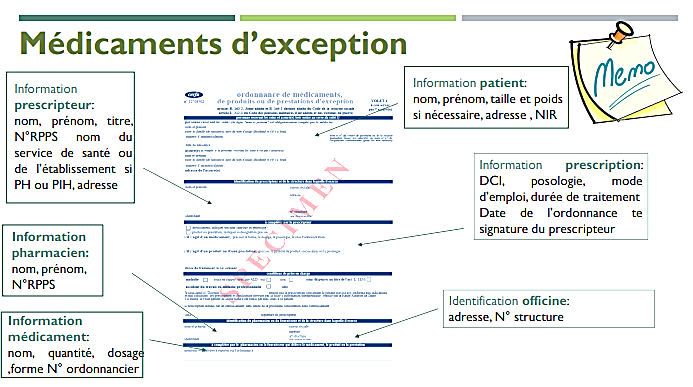
\includegraphics[width=.9\linewidth]{./exception.png}
\end{center}
\end{document}